\documentclass[11pt,a4paper]{article}
\usepackage[utf8]{inputenc}
\usepackage[spanish]{babel}
\usepackage{amsmath}
\usepackage{amsfonts}
\usepackage{amssymb}
\usepackage{braket} % Para notación de Dirac
\usepackage{graphicx}
\usepackage{float}
\usepackage{geometry}
\geometry{left=2.5cm, right=2.5cm, top=2.5cm, bottom=2.5cm}

\title{\textbf{Computación Cuántica: Lista de Ejercicios 01}}
\author{Docente: Raul Huillca Huallparimachi \\ Curso: Computación Cuántica}
\date{29/08/2025}

\begin{document}

\maketitle

\section*{1. Reconocer vectores de probabilidad}

Sea $\Sigma = \{0,1,2,\ldots,9\}$ el conjunto de estados clásicos de un sistema que representa un solo dígito.

\textbf{¿Cuáles de los siguientes vectores son vectores de probabilidad?} Justifique su respuesta.

\begin{enumerate}
    \item $\frac{2}{5}|8\rangle+\frac{1}{5}\left(|3\rangle+|4\rangle+|5\rangle\right)$
    \item $\frac{3}{2}|0\rangle+\frac{1}{2}|1\rangle-|0\rangle$
    \item $\frac{1}{10}\sum_{j=1}^{9}|j\rangle$
    \item $(1-\sqrt{2})|7\rangle+\sqrt{2}|2\rangle$
    \item $\frac{1}{3}|3\rangle+\frac{1}{4}|4\rangle+\frac{5}{12}|5\rangle$
\end{enumerate}

\begin{figure}[H]
    \centering
    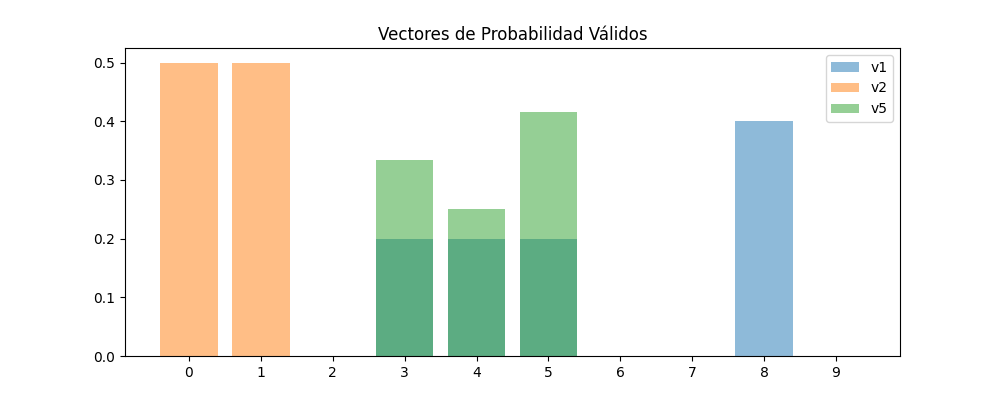
\includegraphics[width=0.75\textwidth]{ej1_prob_vectors.png}
    \caption{Visualización de vectores de probabilidad válidos.}
\end{figure}

\vspace{0.5em}
\textbf{Solución:}
Un vector es de probabilidad si la suma de sus componentes es $1$ y todas sus componentes son $\geq 0$.
\begin{itemize}
    \item \textbf{1. Sí.} $\frac{2}{5} + \frac{1}{5}(1+1+1) = \frac{2}{5} + \frac{3}{5} = 1$. Todas son $\geq 0$.
    \item \textbf{2. Sí.} El vector evaluado es $\left(\frac{3}{2}-1\right)|0\rangle + \frac{1}{2}|1\rangle = \frac{1}{2}|0\rangle + \frac{1}{2}|1\rangle$. La suma es $\frac{1}{2}+\frac{1}{2}=1$.
    \item \textbf{3. No.} La suma es $9 \times \frac{1}{10} = \frac{9}{10} \neq 1$.
    \item \textbf{4. No.} Contiene un componente negativo, ya que $1-\sqrt{2} < 0$.
    \item \textbf{5. Sí.} La suma es $\frac{1}{3} + \frac{1}{4} + \frac{5}{12} = \frac{4}{12} + \frac{3}{12} + \frac{5}{12} = \frac{12}{12} = 1$.
\end{itemize}

\section*{2. Reconocer matrices estocásticas}

Las siguientes matrices son todas matrices de $3\times 3$.

\textbf{Seleccione todas aquellas que sean matrices estocásticas.}

\begin{enumerate}
    \item $|0\rangle\langle0|+|1\rangle\langle1|-|2\rangle\langle2|$
    \item $\begin{pmatrix} \frac{1}{3} & \frac{1}{3} & \frac{1}{3}\\ \frac{1}{4} & \frac{5}{12} & \frac{1}{3}\\ \frac{5}{12} & \frac{1}{3} & \frac{1}{4} \end{pmatrix}$
    \item $\begin{pmatrix} 0 & 1 & 0\\ 0 & 0 & 1\\ 1 & 0 & 0 \end{pmatrix}$
    \item $\frac{1}{3}\left(|0\rangle+|1\rangle+|2\rangle\right)\left(\langle0|+\langle1|+\langle2|\right)$
    \item $\begin{pmatrix} 1 & 1 & 0\\ 0 & 0 & 1\\ 1 & 0 & 0 \end{pmatrix}$
    \item $\begin{pmatrix} 1 & 0 & 0\\ 1 & 0 & 0\\ 0 & 1 & 0 \end{pmatrix}$
\end{enumerate}

\begin{figure}[H]
    \centering
    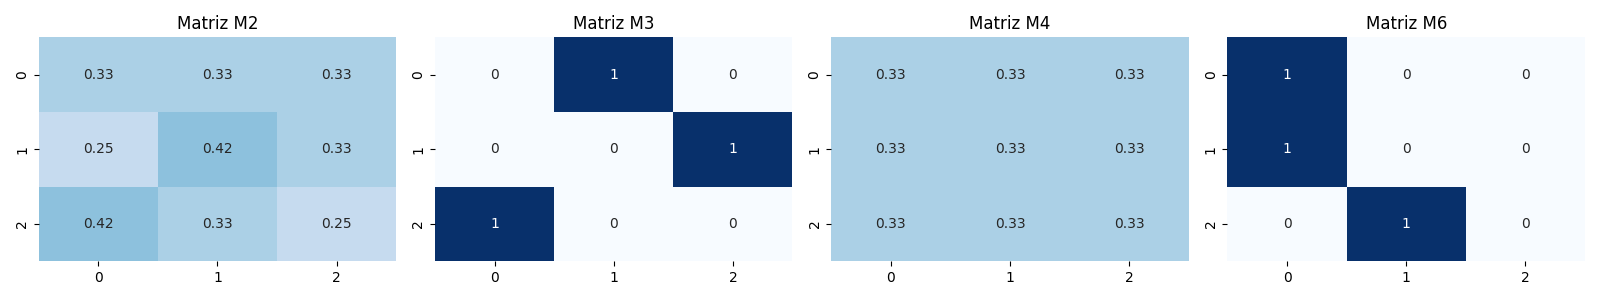
\includegraphics[width=0.9\textwidth]{ej2_stochastic_matrices.png}
    \caption{Matrices estocásticas identificadas representadas como mapas de calor.}
\end{figure}

\vspace{0.5em}
\textbf{Solución:}
Para ser una matriz estocástica (por filas), todas las entradas deben ser $\geq 0$ y la suma de cada fila debe ser $1$.
\begin{itemize}
    \item \textbf{1. No.} Contiene una entrada negativa ($-1$).
    \item \textbf{2. Sí.} Todas las entradas son $\geq 0$. Suma de Fila 1: $\frac{1}{3}+\frac{1}{3}+\frac{1}{3}=1$. Fila 2: $\frac{1}{4}+\frac{5}{12}+\frac{1}{3}=\frac{3+5+4}{12}=1$. Fila 3: $\frac{5}{12}+\frac{1}{3}+\frac{1}{4}=1$.
    \item \textbf{3. Sí.} Es una matriz de permutación, la suma por filas es $1$.
    \item \textbf{4. Sí.} Todas las entradas son $\frac{1}{3}$, la suma por filas es $3 \times \frac{1}{3} = 1$.
    \item \textbf{5. No.} La suma de la primera fila es $1+1+0=2 \neq 1$.
    \item \textbf{6. Sí.} Todas las sumas por fila son $1$.
\end{itemize}

\section*{3. Convertir matriz a notación de Dirac}

Sean $|0\rangle$ y $|1\rangle$ los vectores base estándar para un solo qubit:
$$|0\rangle= \begin{pmatrix} 1\\ 0 \end{pmatrix}, \qquad |1\rangle= \begin{pmatrix} 0\\ 1 \end{pmatrix}$$

¿Cuál de las siguientes es una representación correcta de la matriz
$$M= \begin{pmatrix} 2 & -1\\ -9 & 3 \end{pmatrix}$$
en notación de Dirac? \textbf{Demuestre todas las opciones.}

\begin{enumerate}
    \item $M= 2(2|0\rangle-|1\rangle) (-9\langle0|+3\langle1|)$
    \item $M= 2|0\rangle\langle0| -|0\rangle\langle1| -9|1\rangle\langle0| +3|1\rangle\langle1|$
    \item $M= 2|1\rangle\langle1| -|0\rangle\langle1| -9|1\rangle\langle0| +3|0\rangle\langle0|$
    \item $M= 2|0\rangle\langle0| -|1\rangle\langle0| -9|0\rangle\langle1| +3|1\rangle\langle1|$
    \item $M= 2|00\rangle\langle00| -|01\rangle\langle01| -9|10\rangle\langle10| +3|11\rangle\langle11|$
\end{enumerate}

\vspace{0.5em}
\textbf{Solución:}
La matriz $M$ se puede descomponer en notación de Dirac sumando cada componente $M_{ij} |i\rangle\langle j|$:
$$M = M_{00}|0\rangle\langle0| + M_{01}|0\rangle\langle1| + M_{10}|1\rangle\langle0| + M_{11}|1\rangle\langle1|$$
Reemplazando con los valores de la matriz:
$$M = 2|0\rangle\langle0| - 1|0\rangle\langle1| - 9|1\rangle\langle0| + 3|1\rangle\langle1|$$
Por lo tanto, la opción correcta es la \textbf{2}. Las opciones 1, 3, 4 y 5 al ser desarrolladas no coinciden con esta expresión matricial.

\section*{4. Reconocer vectores de estados cuánticos}

Sea $\Sigma=\{\#,b,c\}$ el conjunto de estados clásicos de un sistema.

\textbf{¿Cuáles de los siguientes son vectores de estados cuánticos?} Seleccione todas las que correspondan.

\begin{enumerate}
    \item $\frac{1}{2} \left( \sqrt{6}|\#\rangle -\sqrt{2}|b\rangle +2i|c\rangle \right)$
    \item $\sqrt{\frac{i}{3}}|c\rangle +\sqrt{\frac{1}{2}}|\#\rangle +\sqrt{\frac{1}{6}}|b\rangle$
    \item $\frac{1}{2} \left( \sqrt{2}|c\rangle -\sqrt{\frac{2}{3}}|\#\rangle +\sqrt{\frac{2i}{3}}|b\rangle \right)$
    \item $\frac{i-\sqrt{3}}{2\sqrt{3}}|c\rangle +\sqrt{\frac{1-i}{12}}|b\rangle +\sqrt{\frac{1}{2}}|\#\rangle$
\end{enumerate}

\begin{figure}[H]
    \centering
    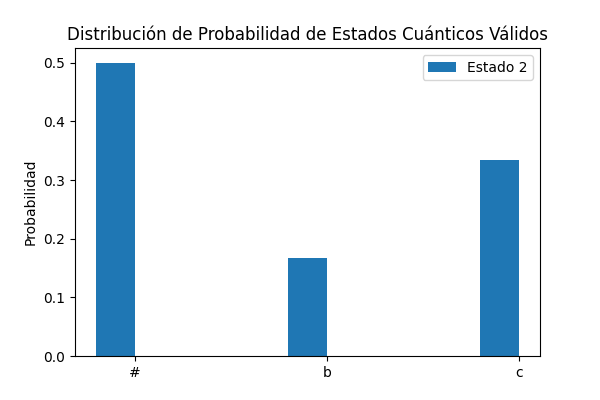
\includegraphics[width=0.75\textwidth]{ej4_quantum_states.png}
    \caption{Distribución de probabilidad de los estados cuánticos válidos.}
\end{figure}

\vspace{0.5em}
\textbf{Solución:}
Para que un vector sea de estado cuántico, su norma al cuadrado debe ser $1$ ($\sum |\alpha_i|^2 = 1$).
\begin{itemize}
    \item \textbf{1. No.} Norma$^2 = \frac{1}{4}\left(|\sqrt{6}|^2 + |-\sqrt{2}|^2 + |2i|^2\right) = \frac{1}{4}(6 + 2 + 4) = 3 \neq 1$.
    \item \textbf{2. Sí.} Norma$^2 = \left|\sqrt{\frac{i}{3}}\right|^2 + \left|\sqrt{\frac{1}{2}}\right|^2 + \left|\sqrt{\frac{1}{6}}\right|^2 = \frac{1}{3} + \frac{1}{2} + \frac{1}{6} = \frac{2+3+1}{6} = 1$.
    \item \textbf{3. No.} Norma$^2 = \frac{1}{4}\left(|\sqrt{2}|^2 + \left|-\sqrt{\frac{2}{3}}\right|^2 + \left|\sqrt{\frac{2i}{3}}\right|^2\right) = \frac{1}{4}\left(2 + \frac{2}{3} + \frac{2}{3}\right) = \frac{10}{12} = \frac{5}{6} \neq 1$.
    \item \textbf{4. No.} Norma$^2 = \left|\frac{i-\sqrt{3}}{2\sqrt{3}}\right|^2 + \left|\sqrt{\frac{1-i}{12}}\right|^2 + \left|\sqrt{\frac{1}{2}}\right|^2 = \frac{1+3}{12} + \frac{\sqrt{2}}{12} + \frac{1}{2} = \frac{5}{6} + \frac{\sqrt{2}}{12} \neq 1$.
\end{itemize}

\section*{5. Orden alfabético de productos cartesianos}

Sea $\Gamma=\{1,2,3,4\}$ ordenado como está escrito, con $1$ primero.

\textbf{¿Cuál es el elemento número 12 del conjunto $\Gamma\times\Gamma$ ordenado alfabéticamente?}

\vspace{0.5em}
\textbf{Solución:}
El conjunto $\Gamma \times \Gamma$ tiene $4 \times 4 = 16$ elementos ordenados de la siguiente forma:
$$(1,1), (1,2), (1,3), (1,4),$$
$$(2,1), (2,2), (2,3), (2,4),$$
$$(3,1), (3,2), (3,3), (3,4), \dots$$
Como cada número inicial agrupa $4$ elementos, el elemento número 12 es el último del tercer grupo, es decir, \textbf{$(3,4)$}.

\section*{6. Calcular productos tensoriales}

Se tienen los siguientes vectores:
$$|u\rangle= \begin{pmatrix} -2\\ 1 \end{pmatrix}, \qquad |v\rangle= \begin{pmatrix} 1\\ 0\\ 1 \end{pmatrix}$$
$$|w\rangle= \begin{pmatrix} 4\\ 1 \end{pmatrix}, \qquad |x\rangle= \begin{pmatrix} \frac{1}{2}\\ \frac{1}{2}\\ \frac{1}{2} \end{pmatrix}$$

Calcular el siguiente producto tensorial:
$$|u\rangle\otimes|v\rangle -\frac{2}{3} |w\rangle\otimes|x\rangle$$

\vspace{0.5em}
\textbf{Solución:}
Calculamos primero el producto tensorial $|u\rangle\otimes|v\rangle$:
$$|u\rangle\otimes|v\rangle = \begin{pmatrix} -2 \\ 1 \end{pmatrix} \otimes \begin{pmatrix} 1 \\ 0 \\ 1 \end{pmatrix} = \begin{pmatrix} -2(1) \\ -2(0) \\ -2(1) \\ 1(1) \\ 1(0) \\ 1(1) \end{pmatrix} = \begin{pmatrix} -2 \\ 0 \\ -2 \\ 1 \\ 0 \\ 1 \end{pmatrix}$$

Luego calculamos $\frac{2}{3}|w\rangle\otimes|x\rangle$:
$$\frac{2}{3}|w\rangle\otimes|x\rangle = \frac{2}{3} \begin{pmatrix} 4 \\ 1 \end{pmatrix} \otimes \begin{pmatrix} 1/2 \\ 1/2 \\ 1/2 \end{pmatrix} = \frac{2}{3} \begin{pmatrix} 2 \\ 2 \\ 2 \\ 1/2 \\ 1/2 \\ 1/2 \end{pmatrix} = \begin{pmatrix} 4/3 \\ 4/3 \\ 4/3 \\ 1/3 \\ 1/3 \\ 1/3 \end{pmatrix}$$

Restando ambos resultados obtenemos:
$$|u\rangle\otimes|v\rangle - \frac{2}{3} |w\rangle\otimes|x\rangle = \begin{pmatrix} -2 - 4/3 \\ 0 - 4/3 \\ -2 - 4/3 \\ 1 - 1/3 \\ 0 - 1/3 \\ 1 - 1/3 \end{pmatrix} = \begin{pmatrix} -10/3 \\ -4/3 \\ -10/3 \\ 2/3 \\ -1/3 \\ 2/3 \end{pmatrix}$$

\end{document}
